\documentclass[solution,addpoints,12pt]{exam}
\printanswers
\usepackage{amsmath,amssymb}
\usepackage{multirow}
\usepackage{enumitem}
\usepackage[colorlinks=true, linkcolor=blue, urlcolor=blue]{hyperref}
\newcommand{\RP}{\ensuremath{\mathsf{RP}}}
\newcommand{\expect}[1]{\ensuremath{\mathbb{E}[#1]}}
\newcommand{\dx}{\mathrm{d}x}
\usepackage{graphicx}
\pointpoints{mark}{marks}
\usepackage{caption}
\usepackage{verbatim}

\begin{document}

\hrule
\vspace{1mm}
\noindent 
\begin{center}
{\Large CS6700 : Reinforcement Learning} \\
{\large Written Assignment \#3}
\end{center}
%\hfill Release date: 21 Jan, 2017, 12:00 pm}
\vspace{1mm}
\noindent 
{\large \hfill Deadline: ??}

\vspace{2mm}
\hrule

{\small

\begin{itemize}\itemsep0mm
\item This is an individual assignment. Collaborations and discussions are strictly
prohibited.
\item Be precise with your explanations. Unnecessary verbosity will be penalized.
\item Check the Moodle discussion forums regularly for updates regarding the assignment.
\item \textbf{Please start early.}
%\item Turn in \textbf{only the answers} on Turnitin.
\end{itemize}
}

\hrule

\vspace{3mm}
\noindent {\sc Author :} Name. \\[1mm]
\noindent {\sc Roll Number :} \\
%\hrule


\begin{questions}
\question[3] Consider the problem of solving POMDPs using Deep Reinforcement Learning. Can you think of ways to modify the standard DQN architecture to ensure it can remember histories of states. Does the experience replay also need to be modified? Explain.

\begin{solution}
Ref: \url{ http://cs229.stanford.edu/proj2015/363_report.pdf} \\
In deep Q learning, a neural network is used to approximate the POMDP Q-values. For POMDP, the Q values are parameterized by either the belief and the action Q(b,a) or an action-observation history h and Q(h,a). The modified Q-values can be learned by a neural network that is characterized by weights and biases combined denoted as $\theta$. Q values will be $Q(b,a|\theta)$. The standard update of Q values may lead to divergence. Such issues is resolved by experience replay tuples (b,a,r,b′) which are recorded in a reply memory. The aim of replay is to stabilize the learning by drawing samples uniformly.

\begin{center}
	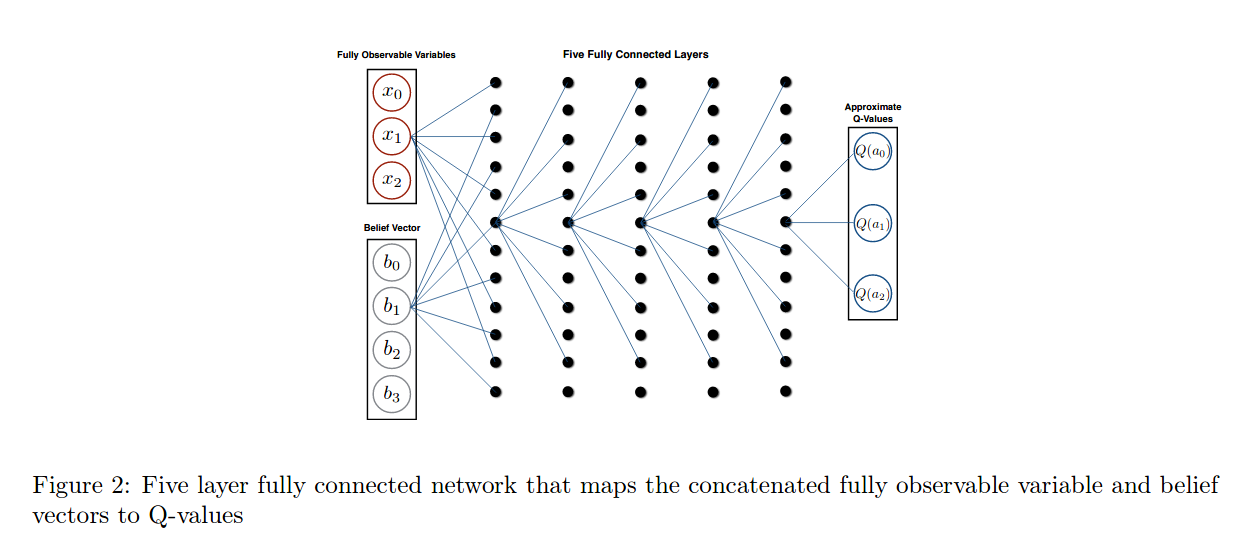
\includegraphics[trim={0cm 0cm 0cm 0cm},clip,scale=0.2]{DQN.png}\label{DQN}
\end{center}

Apart from this, a separate target network is used update state targets to the main network.  An adaptive learning method can be used  to  regulate and adjustment the parameter rate  of  the  network. 

\textbf{Changes in architecture:} \\
The changed architecture of DQN is given in figure-\ref{DQN}. In architecture, simulator is used to populate and experience reply dataset. The input layer consists the belief of the agent and fully observable state variables which generalize the representation of problems. The agent may have some knowledge of the system state known as mixed observability MDPs(MDOMPs). 
\textbf{A similar architecture was used for training the DQN on action observation histories which requires the manipulation of experience reply for efficient use of reply.}  The fully observable state variables are used as inputs to the network. The current formulation uses a fully connected network that either takes the fully observable state variables and the belief or just the belief  and outputs a value approximation.
\end{solution}


\question[4] Exploration is often ameliorated by the use of counts over the various states. For example, one could maintain a visitation count $N(s)$, for every state and use the same to generate an intrinsic reward ($r_i(s)$) for visiting that state.
\[ r_i(s) = \tau \times \frac{1}{N(s)} \]
However, it is intractable to maintain these counts in high-dimensional spaces, since the count values will be zero for a large fraction of the states. Can you suggest a solution(s) to handle this scenario? How can you maintain an approximation of the counts for a large number of states and possibly generalize to unseen states?

\begin{solution}
Ref: \url{http://surl.tirl.info/proceedings/SURL-2017_paper_5.pdf} \\
The solution to this problem is count-based exploration algorithm. The proposed algorithm uses linear function approximation(LFA). 
The key idea behind the algorithm is to exploit the feature map that is uses of value function approximation, and construct a density model over the transformed feature space. The model assigns higher probability to state feature vectors that share features with visited states.

The algorithm is called $\phi$-Exploration Bonus algorithm. A generalized count is a novelty measure that quantifies how dissimilar a state is from those already visited. $\phi_t = \phi(s_t)$ denote the state feature vector observed at time t. We denote the sequence of observed feature vectors after t timesteps by $\phi_{1:t}\in T_t$, and denote the set of all finite sequences of feature vectors by $T^*$. $\phi_{1:t}\phi$ denote the sequence where $\phi_{1:t}$ is followed by $\phi$. 
$\rho_t(\phi)$ be the feature visit density after observation of $\phi_{1:t}$. $\rho'_t(\phi)$ density after observation of $\phi_{1:t}\phi$. The pseudocount $N_t^\phi$ is defined as,
\begin{equation}
	N^\phi_t = \frac{\rho_t(\phi(s))(1-\rho'_t(\phi(s)))}{\rho'_t(\phi(s))-\rho_t(\phi(s))}
\end{equation}
By setting the hyper parameter as $\beta$.  The sample reward is defined as,
\begin{equation}
R_t(s,a) = \frac{\beta}{\sqrt{N^\phi_t(s)}}
\end{equation} 
The bonus is added to reward $r_t$. The trained agent augmented reward $r^+_t$ can be obtained using any value based RL algo.
\begin{equation}
r^+_t = r_t + R_t(s,a)
\end{equation}  Due to functional transformation the cost of method is independent from size of the action space.
\end{solution}
\question[5] Suppose that the MDP defined on the observation space is k-th order Markov, i.e. remembering the last k observations is enough to predict the future. 
Consider using a belief state based approach for solving this problem. For any starting state and initial belief, the belief distribution will localize to the right state after k updates, i.e., the true state the agent is in will have a probability of 1 and the other states will have a probability of 0. Is this statement true or false? Explain your answer. 

\begin{solution}
If the information obtained by all states is correct then for $k^{th}$ order Markov chain last k observation is enough to predict the future.  
The example explained in the lecture have possible. 
\begin{center}
	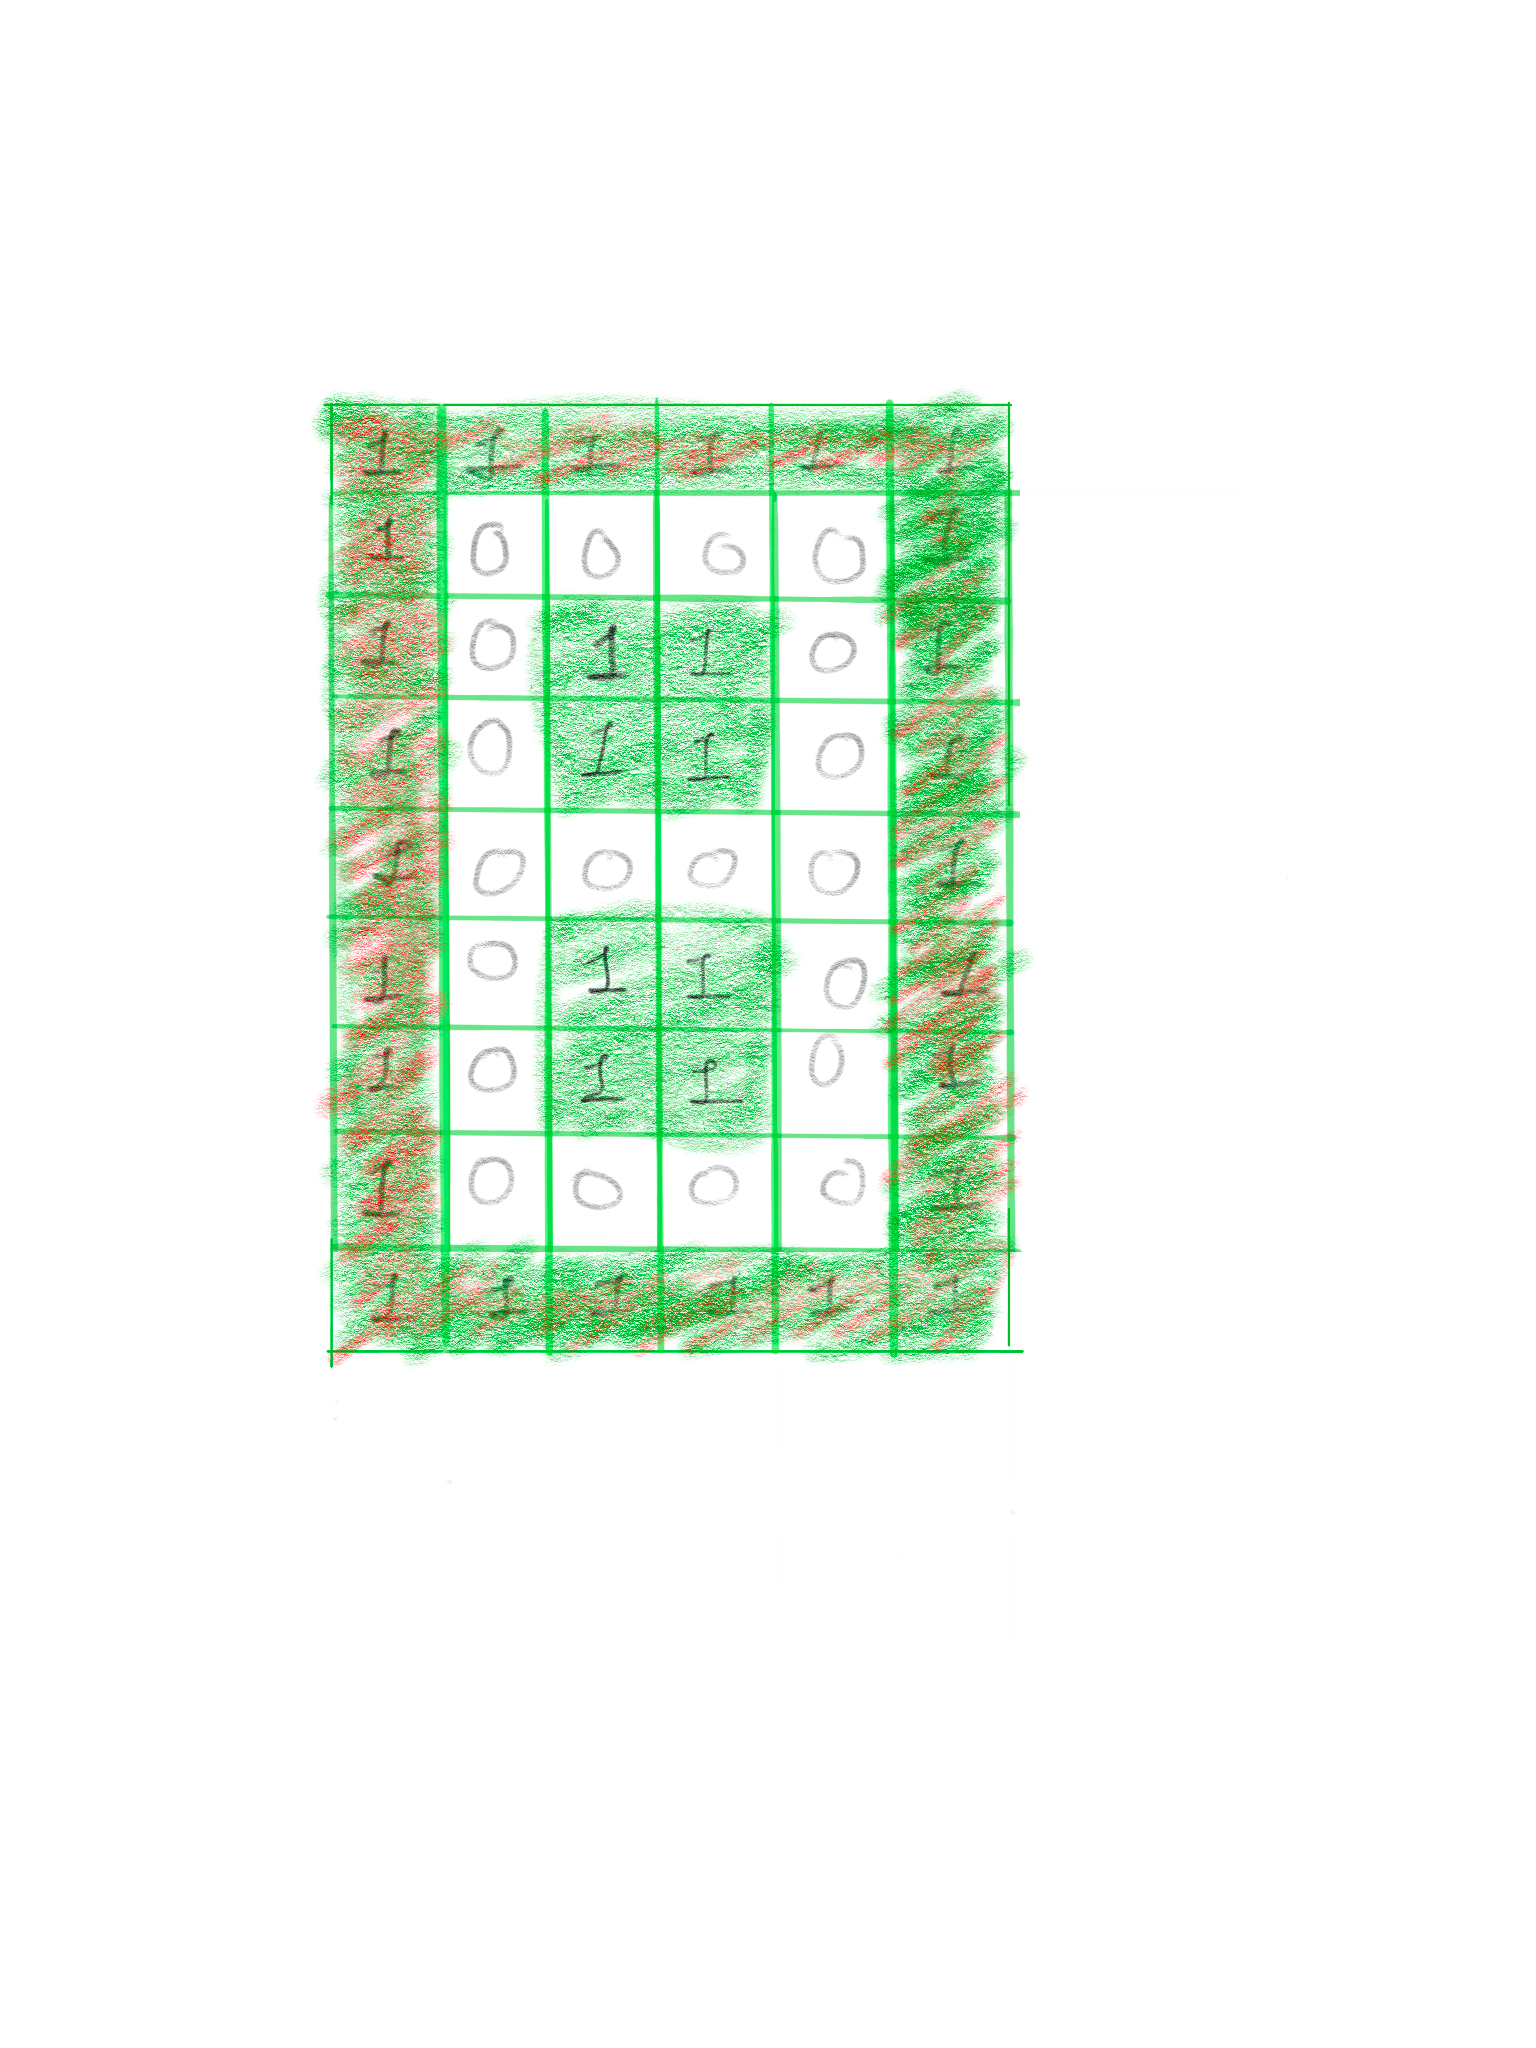
\includegraphics[trim={10cm 20cm 19cm 14cm},clip,scale=0.2]{belief.png}\label{grid}
\end{center}

The Grid world is given in fig-\ref{grid}. Each cell with 0 indicates clear or approachable state and 1 indicates(green colour) are obstacles. Green and Red colour cell indicates wall. The location of state is give based on its neighbor cell. The state numbering starts from north and goes by following clockwise direction. States: 0001, 1010, 0101, 1100, 0110, 0011, 0100, 1001 have its count respectively 1, 6, 8, 1, 1, 1, 1, 1.

\textbf{Let's take example of to reach 1001.}  There are many ways to reach at that spot. But if we know certain history then it attainable to reach desired state with Pr=1. Initial state have some initial belief p(s). As more observation is added in terms of history, the belief about the state space keeps getting more focused.  

\end{solution}


\question[3]
Q-MDPs are a technique for solving the problem of behaving in POMDPs. The behavior produced by this approximation would not be optimal. In what sense is it not optimal?  Are there circumstances under which it can be optimal?

\begin{solution}
	In Q-MDP we have solved the problem assuming that we access to state at that point. But to solve the problem later, by heuristic approach to get the execution policy. The obtained execution policy obtained by heuristic way might not be optimal as heuristic might have uncertainty in states and there might be better action to pick in terms of total reward obtained. so,\textbf{ execution policy obtained by heuristic might have uncertainty and this lead to sub-optimal approximation.}
	
	If we solve the POMDP directly then there are chance to get optimal scenario given states are known. Known states and desired action gives next states and which makes policy deterministic. \textbf{Using the simplex belief states and relation between value function gives efficient way to solve POMDP directly to learn policy from history such deterministic scenario makes approximation optial.}
\end{solution}

\question[3] What are some advantages and disadvantages of A3C over DQN? What are some potential issues that can be caused by asynchronous updates in A3C?

\begin{solution}
In DQN, a single agent interacts with a single environment. whereas, A3C asynchronously launches many workers  based on efficiency of CPU. All of them interact with their own environment. Every worker instance also has their own environment which gives more diverse data. This approach makes network robust and gives good results.\\
\textbf{Advantages of A3C:}
 \subitem --- By asynchronously launching more workers gives more training data, which makes the collection of the data faster.
 \subitem --- As every worker have different environment, the data obtained will be more diverse. 
 \subitem --- The variation in data makes process more efficient and gives better result. 
 
 \textbf{Disadvantages of A3C:}
 \subitem --- More computational effort 
 \subitem --- Some similar workers may generated repeated samples which may cause bias in the learning.
 
 \textbf{Potential issues that can be caused by asynchronous updates in A3C:}
\subitem ---  some workers (copies of the Agent) will be playing with older version of the parameters because of the asynchronous nature and the aggregate update might not be optimal.


\end{solution}

\question[6] There are a variety of very efficient heuristics available for solving deterministic travelling salesman problems. We would like to take advantage of such heuristics in solving
certain classes of large scale navigational problems in stochastic domains. These problems involve navigating from one well demarcated region to another. For e.g., consider
the problem of delivering mail to the office rooms in a multi storey building.

\begin{parts}
    \part[4] Outline a method to achieve this, using concepts from hierarchical RL.
    \begin{solution}
    
    \end{solution}
    \part[2] What problems would such an approach encounter?
    \begin{solution}
    
    \end{solution}
\end{parts}

\question[6] This question may require you to refer to \href{this}{https://link.springer.com/content/pdf/10.1007/BF00114727.pdf} paper on average reward RL. Consider the 3 state MDP shown in Figure \ref{fig:avg}.  Mention the recurrent class for each such policies. In the average reward setting, what are the corresponding $\rho^{\pi}$ for each such policy ? Furthermore, which of these policies are gain optimal ? 
    \begin{parts}
        \part[3] What are the different deterministic uni-chain policies present ?
        \part[3] In the average reward setting, what are the corresponding $\rho^{\pi}$ for each such policy ? Furthermore, which of these policies are gain optimal ? 
    \end{parts}

    \begin{figure}[h]
        \centering
        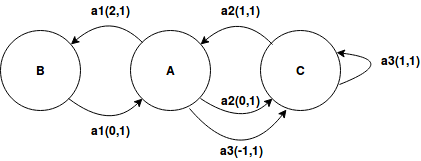
\includegraphics[scale=0.6]{average_reward.png}
        \caption{Notation : action(reward, transition probability). Example : a1(3, 1) refers to action a1 which results in a transition with reward +3 and probability 1}
        \label{fig:avg}
    \end{figure}

\end{questions}


\end{document}